\documentclass[10pt,a4paper]{article}
\usepackage[a4paper,margin=1.45cm,top=1.55cm,bottom=1.55cm]{geometry}
\usepackage{fontspec}
\setmainfont{Segoe UI}
\setmonofont{Consolas}
\usepackage[italian]{babel}
\usepackage{xcolor}
\usepackage{graphicx}
\usepackage{booktabs}
\usepackage{tabularx}
\usepackage{array}
\usepackage{enumitem}
\usepackage{needspace}
\usepackage{hyperref}
\usepackage{fancyhdr}
\usepackage{tikz}
\usetikzlibrary{positioning}
\usepackage[most]{tcolorbox}
\tcbuselibrary{listings,breakable,skins}

\definecolor{navy}{HTML}{17324D}
\definecolor{accent}{HTML}{007ACC}
\definecolor{softblue}{HTML}{EAF4FB}
\definecolor{softgreen}{HTML}{EAF7EF}
\definecolor{softorange}{HTML}{FFF3E5}
\definecolor{linegray}{HTML}{D9E1E8}
\definecolor{vsbg}{HTML}{FFFFFF}
\definecolor{vsfg}{HTML}{1F1F1F}
\definecolor{vsblue}{HTML}{0000FF}
\definecolor{vstype}{HTML}{267F99}
\definecolor{vsstring}{HTML}{A31515}
\definecolor{vscomment}{HTML}{008000}
\definecolor{vsnumber}{HTML}{098658}
\definecolor{vspurple}{HTML}{AF00DB}

\hypersetup{colorlinks=true,linkcolor=accent,urlcolor=accent}
\pagestyle{fancy}
\fancyhf{}
\lhead{Java Collections Framework}
\rhead{Scheda da stampare}
\cfoot{\thepage}
\renewcommand{\headrulewidth}{0.4pt}
\setlength{\parindent}{0pt}
\setlength{\parskip}{4pt}
\setlist[itemize]{leftmargin=5mm,itemsep=1pt,topsep=2pt}

\lstdefinestyle{vscode}{
  language=Java,
  basicstyle=\ttfamily\small\color{vsfg},
  keywordstyle=\bfseries\color{vsblue},
  keywordstyle=[2]\color{vstype},
  stringstyle=\color{vsstring},
  commentstyle=\itshape\color{vscomment},
  numberstyle=\tiny\color{vsnumber},
  morekeywords=[2]{String,Integer,Double,Person,List,ArrayList,LinkedList,Set,HashSet,TreeSet,Map,HashMap,TreeMap,Queue,Deque,Iterator,Collection,Comparable,Comparator,Collections,Arrays,Map.Entry,Stream,Collectors,Optional,Objects},
  showstringspaces=false,
  columns=fullflexible,
  keepspaces=true,
  tabsize=4,
  breaklines=true,
  numbers=left,
  numbersep=7pt,
  xleftmargin=4mm,
  frame=none
}

\newtcblisting{codebox}[1]{
  enhanced,
  listing only,
  listing options={style=vscode},
  colback=vsbg,
  colframe=accent,
  coltitle=white,
  fonttitle=\bfseries,
  title={#1},
  arc=2mm,
  boxrule=0.7pt,
  left=1mm,right=1mm,top=1mm,bottom=1mm,
  before skip=5pt,after skip=7pt
}

\newtcolorbox{concept}[2][]{
  enhanced,colback=softblue,colframe=accent,
  title={#2},fonttitle=\bfseries,coltitle=navy,
  arc=2mm,boxrule=.6pt,#1
}
\newtcolorbox{difference}[2][]{
  enhanced,colback=softgreen,colframe=green!55!black,
  title={#2},fonttitle=\bfseries,coltitle=green!25!black,
  arc=2mm,boxrule=.6pt,#1
}
\newcommand{\cmd}[1]{\texttt{#1}}
\newcommand{\complexity}[1]{\textcolor{accent}{\textbf{#1}}}
\newcommand{\topicsection}[1]{\Needspace{12\baselineskip}\section{#1}}
\newcommand{\topicsubsection}[1]{\Needspace{10\baselineskip}\subsection{#1}}
\newenvironment{topicblock}{%
  \par\medskip\noindent\begin{minipage}{\textwidth}%
}{%
  \end{minipage}\par\medskip%
}

\begin{document}

\begin{titlepage}
\centering
\vspace*{1.2cm}
{\Huge\bfseries\color{navy} Java Collections Framework\par}
\vspace{.35cm}
{\LARGE Gerarchia, metodi distintivi e codice reale\par}
\vspace{.5cm}
{\large Scheda di ripasso pronta da stampare\par}
\vspace{1cm}
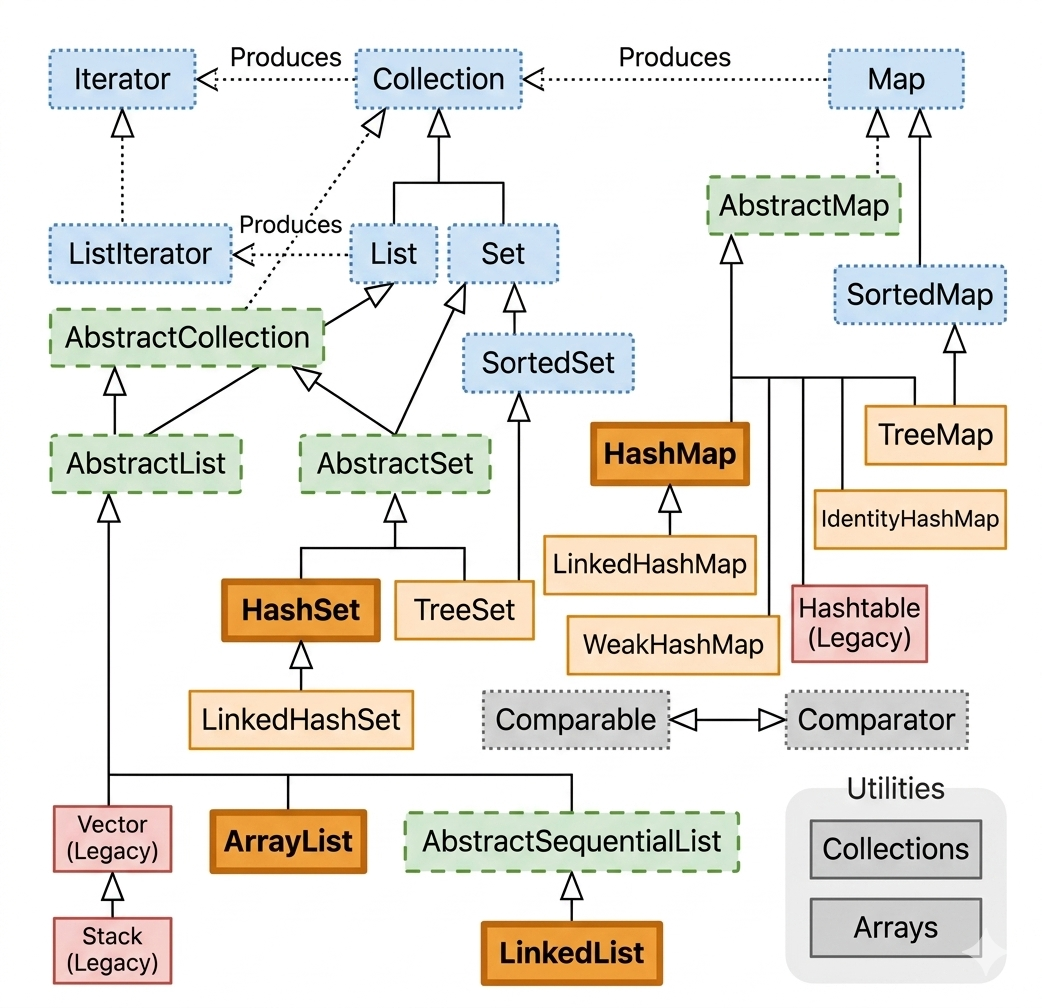
\includegraphics[width=.79\textwidth]{Gemini_Generated_Image_pjh5i4pjh5i4pjh5.png}
\vfill
\begin{tcolorbox}[width=.92\textwidth,colback=softorange,colframe=orange!70!black,arc=2mm]
\textbf{Idea chiave:} dichiara le variabili usando l'interfaccia necessaria, e scegli la classe concreta in base a ordine, duplicati e prestazioni.

\centering\texttt{List<String> nomi = new ArrayList<>();}
\end{tcolorbox}
\vfill
{\small Materiale basato sulle dispense del corso e integrato con gli esercizi degli esami precedenti.}
\end{titlepage}

\tableofcontents
\newpage

\topicsection{Come leggere la gerarchia}

\begin{concept}{Interfacce, classi astratte e classi concrete}
\begin{itemize}
\item \textbf{Blu nell'immagine}: interfacce, cioè contratti che possono essere usati come tipi.
\item \textbf{Verde}: classi astratte, cioè basi comuni per implementare nuove collezioni.
\item \textbf{Arancione}: classi concrete, normalmente istanziate con \cmd{new}.
\item \textbf{Map è separata da Collection}: gestisce associazioni chiave--valore, non una sequenza di elementi singoli.
\end{itemize}
\end{concept}

\begin{center}
\begin{tikzpicture}[node distance=8mm and 12mm,every node/.style={draw,rounded corners,minimum width=25mm,minimum height=8mm,font=\small},arr/.style={->,thick,accent}]
\node (it) {Iterable<E>};
\node (co) [below=of it] {Collection<E>};
\node (li) [below left=of co] {List<E>};
\node (se) [below=of co] {Set<E>};
\node (qu) [below right=of co] {Queue<E>};
\node (map) [right=35mm of co] {Map<K,V>};
\draw[arr] (co)--(it); \draw[arr] (li)--(co); \draw[arr] (se)--(co); \draw[arr] (qu)--(co);
\node[draw=none,below=1mm of map,font=\footnotesize] {gerarchia separata};
\end{tikzpicture}
\end{center}

\begin{topicblock}
\topicsection{Iterable e Iterator}

\begin{concept}{Ruolo e comandi}
\cmd{Iterable<E>} espone \cmd{iterator()} e può quindi essere usato in un
\cmd{for-each}. L'oggetto \cmd{Iterator<E>} mantiene la posizione raggiunta
durante la visita.

\textbf{Comandi:} \cmd{iterator()}, \cmd{hasNext()}, \cmd{next()},
\cmd{remove()} (se supportato dall'iteratore) e \cmd{forEach(action)}.
\end{concept}

\begin{codebox}{Visita manuale con Iterator}
List<String> names = Arrays.asList("Anna", "Luca", "Sara");
Iterator<String> iterator = names.iterator();

// L'Iterator ricorda autonomamente la posizione corrente
while (iterator.hasNext()) {
    String name = iterator.next();
    System.out.println(name); // Anna, poi Luca, poi Sara
}

// Forma equivalente e più comune:
for (String name : names) {
    System.out.println(name);
}

// Lambda: esegue println una volta per ogni elemento
names.forEach(name -> System.out.println(name));

// Riferimento a metodo: forma abbreviata equivalente
names.forEach(System.out::println);
\end{codebox}

\begin{difference}{Da ricordare}
\cmd{Iterable} garantisce soltanto la possibilità di scorrere gli elementi:
non possiede \cmd{size()} o \cmd{add()}. Questi metodi sono definiti da
\cmd{Collection}.
\end{difference}

\end{topicblock}
\begin{topicblock}
\topicsection{Collection: operazioni comuni}

\begin{concept}{Metodi usati nel corso}
\begin{tabularx}{\textwidth}{>{\ttfamily}l X}
add(e), addAll(c) & aggiungono uno o più elementi; restituiscono se la collezione è cambiata \\
remove(e), removeAll(c) & rimuovono elementi; restituiscono se la collezione è cambiata \\
retainAll(c) & conserva soltanto gli elementi presenti anche in \cmd{c} \\
contains(e), containsAll(c) & verificano la presenza di uno o più elementi \\
size(), isEmpty() & restituiscono la dimensione e indicano se la collezione è vuota \\
clear() & elimina tutti gli elementi \\
toArray(), iterator() & convertono in array o permettono la visita \\
\end{tabularx}
\end{concept}

\begin{codebox}{Programmare verso l'interfaccia Collection}
Collection<Integer> values = new ArrayList<>();
values.addAll(Arrays.asList(1, 3, 5, 7));

boolean added = values.add(9);    // true: 9 viene inserito
boolean removed = values.remove(3); // true: 3 era presente
boolean found = values.contains(5); // true

System.out.println(values);       // [1, 5, 7, 9]
System.out.println(values.size()); // 4

for (int value : values) {
    System.out.println(value);
}
\end{codebox}

\end{topicblock}
\topicsection{List, ArrayList e LinkedList}

\begin{topicblock}
\topicsubsection{List}
\begin{concept}{Metodi d'istanza distintivi di List}
Una \cmd{List} ammette duplicati, conserva l'ordine degli elementi e permette
l'accesso tramite indice. Il primo indice è zero.

\begin{tabularx}{\textwidth}{>{\ttfamily\small}p{4cm} X}
get(index) & legge l'elemento in posizione \cmd{index} \\
set(index, value) & sostituisce e restituisce il vecchio elemento \\
add(index, value) & inserisce spostando a destra gli elementi successivi \\
remove(index) & rimuove per posizione e restituisce l'elemento rimosso \\
remove(value) & rimuove la prima occorrenza del valore e restituisce un booleano \\
indexOf(value) & prima posizione, oppure $-1$ \\
lastIndexOf(value) & ultima posizione, oppure $-1$ \\
subList(from, to) & vista dall'indice \cmd{from} incluso a \cmd{to} escluso \\
listIterator() & iteratore bidirezionale specifico delle liste \\
\end{tabularx}
\end{concept}

\begin{codebox}{Operazioni distintive di List}
List<String> list = new ArrayList<>(
    Arrays.asList("A", "B", "A")
); // ordine e duplicati conservati

String second = list.get(1);      // "B"
String old = list.set(1, "X");    // old = "B"
list.add(1, "C");                 // [A, C, X, A]
int firstA = list.indexOf("A");   // 0
int lastA = list.lastIndexOf("A");// 3
List<String> part = list.subList(1, 3); // [C, X]
// part è una vista: le modifiche si riflettono anche su list
\end{codebox}

\begin{difference}{Attenzione a remove con List<Integer>}
\cmd{numbers.remove(1)} interpreta \cmd{1} come indice.\\
Per rimuovere il valore intero \cmd{1} bisogna scrivere
\cmd{numbers.remove(Integer.valueOf(1))}.
\end{difference}

\end{topicblock}
\begin{topicblock}
\topicsubsection{ArrayList}
\begin{difference}{Quando sceglierla}
Array dinamico: \cmd{get(i)} e \cmd{set(i,e)} sono \complexity{O(1)};
\cmd{add(e)} in fondo è mediamente \complexity{O(1)}, mentre inserimenti e
rimozioni nel mezzo sono \complexity{O(n)}. È la scelta iniziale più comune
quando serve una lista.

\textbf{Metodi propri:}
\cmd{ensureCapacity(n)} prepara spazio senza cambiare \cmd{size()};
\cmd{trimToSize()} riduce la capacità interna agli elementi presenti.
Tutti gli altri comandi principali provengono da \cmd{List}.
\end{difference}

\begin{codebox}{ArrayList: capacità e accesso rapido}
ArrayList<String> students = new ArrayList<>();
students.ensureCapacity(30); // capacità >= 30, ma size() == 0

students.add("Anna");
students.add("Luca");
students.add("Sara");

String first = students.get(0); // accesso O(1): "Anna"
students.remove(1);              // [Anna, Sara]
students.trimToSize();           // riduce solo lo spazio interno
\end{codebox}

\end{topicblock}
\begin{topicblock}
\topicsubsection{LinkedList, Queue e Deque}
\begin{difference}{Quando sceglierla}
Lista doppiamente concatenata: l'accesso per indice è \complexity{O(n)},
mentre inserimenti e rimozioni alle estremità sono \complexity{O(1)}.
Implementa sia \cmd{List} sia \cmd{Deque}.
\end{difference}

\begin{concept}{Metodi d'istanza di Queue e Deque}
\begin{tabularx}{\textwidth}{>{\ttfamily\small}p{4cm} X}
offer(e) & prova a inserire in coda; restituisce \cmd{false} se non può \\
poll() & legge e rimuove la testa; \cmd{null} se vuota \\
peek() & legge la testa senza rimuoverla; \cmd{null} se vuota \\
remove() / element() & come \cmd{poll}/\cmd{peek}, ma lanciano eccezione se vuota \\
addFirst(e), addLast(e) & inseriscono a una delle estremità \\
pollFirst(), pollLast() & rimuovono da un'estremità; \cmd{null} se vuota \\
peekFirst(), peekLast() & leggono un'estremità senza rimuovere \\
push(e), pop() & uso LIFO: inseriscono e rimuovono dalla testa \\
\end{tabularx}
\end{concept}

\begin{codebox}{LinkedList usata come coda FIFO}
Queue<String> queue = new LinkedList<>();
queue.offer("A");
queue.offer("B");
queue.offer("C"); // ingresso: A, B, C

String first = queue.peek(); // "A", la coda non cambia
String out1 = queue.poll();  // esce "A"
String out2 = queue.poll();  // esce "B"
System.out.println(queue);   // [C]
\end{codebox}

\begin{codebox}{Deque usata come pila LIFO}
Deque<String> deque = new LinkedList<>();
deque.addLast("B");  // [B]
deque.addLast("C");  // [B, C]
deque.push("A");     // [A, B, C]: equivale ad addFirst

String top = deque.pop();        // "A", resta [B, C]
String last = deque.removeLast();// "C", resta [B]
\end{codebox}

\end{topicblock}
\topicsection{Set, HashSet e TreeSet}

\begin{topicblock}
\topicsubsection{Set}
\begin{concept}{Collezione senza duplicati}
\cmd{Set} non aggiunge molti metodi a \cmd{Collection}, ma ne cambia il
contratto: non ammette duplicati e non possiede indici.
\cmd{HashSet} riconosce i duplicati tramite \cmd{equals}/\cmd{hashCode};
\cmd{TreeSet} usa invece \cmd{compareTo} o il \cmd{Comparator}.

\textbf{Metodi usati:}
\cmd{add}, \cmd{addAll}, \cmd{remove}, \cmd{contains}, \cmd{size},
\cmd{isEmpty}, \cmd{clear}, \cmd{iterator}. \cmd{add(e)} restituisce
\cmd{false} quando l'elemento era già presente.
\end{concept}

\end{topicblock}
\begin{topicblock}
\topicsubsection{HashSet}
\begin{difference}{Caratteristiche}
Non garantisce alcun ordine di iterazione. \cmd{add}, \cmd{remove} e
\cmd{contains} costano mediamente \complexity{O(1)}. Usa \cmd{hashCode()}
per restringere la ricerca ed \cmd{equals()} per verificare l'uguaglianza.
\end{difference}

\begin{codebox}{HashSet: unicità e ricerca rapida}
Set<String> tags = new HashSet<>();
boolean first = tags.add("java");  // true
boolean second = tags.add("oop");  // true
boolean duplicate = tags.add("java"); // false

System.out.println(tags.size()); // 2
System.out.println(tags.contains("oop")); // true
tags.remove("oop");              // resta soltanto "java"

// L'ordine di stampa non è garantito
System.out.println(tags);
\end{codebox}

\end{topicblock}
\begin{topicblock}
\topicsubsection{TreeSet}
\begin{difference}{Caratteristiche}
Mantiene gli elementi ordinati secondo l'ordine naturale
(\cmd{Comparable}) oppure secondo un \cmd{Comparator}. Le operazioni
principali costano \complexity{O(log n)}. Implementa \cmd{NavigableSet}.
\end{difference}

\begin{concept}{Metodi d'istanza distintivi di TreeSet}
\begin{tabularx}{\textwidth}{>{\ttfamily\small}p{4cm} X}
first(), last() & minimo e massimo; eccezione se il set è vuoto \\
lower(e), higher(e) & elemento strettamente minore o maggiore \\
floor(e), ceiling(e) & minore/maggiore ammettendo anche l'uguaglianza \\
pollFirst(), pollLast() & rimuovono e restituiscono minimo o massimo; \cmd{null} se vuoto \\
headSet(to) & vista degli elementi minori di \cmd{to} \\
tailSet(from) & vista degli elementi maggiori o uguali a \cmd{from} \\
subSet(from, to) & vista da \cmd{from} incluso a \cmd{to} escluso \\
descendingSet() & vista con ordinamento inverso \\
\end{tabularx}
\end{concept}

\begin{codebox}{TreeSet: ordine e ricerca per vicinanza}
TreeSet<Integer> numbers = new TreeSet<>();
numbers.addAll(Arrays.asList(40, 10, 30, 20, 20));

System.out.println(numbers);     // [10, 20, 30, 40]
// Ordinato automaticamente e senza duplicati

System.out.println(numbers.lower(20));  // 10: strettamente <
System.out.println(numbers.floor(20));  // 20: <=
System.out.println(numbers.ceiling(25));// 30: >=
System.out.println(numbers.higher(30)); // 40: strettamente >
\end{codebox}

\end{topicblock}
\topicsection{Map, HashMap e TreeMap}

\begin{topicblock}
\topicsubsection{Map}
\begin{concept}{Coppie chiave--valore}
\cmd{Map<K,V>} non estende \cmd{Collection}: associa ogni chiave a un valore.
Le chiavi sono uniche; una nuova chiamata a \cmd{put} con una chiave già
presente sostituisce il valore precedente.

\begin{tabularx}{\textwidth}{>{\ttfamily\small}p{5.5cm} X}
put(key, value) & inserisce e restituisce il vecchio valore \\
putAll(map) & copia tutte le associazioni \\
get(key) & valore associato; \cmd{null} se la chiave manca o è associata a \cmd{null} \\
getOrDefault(key, def) & valore associato, oppure \cmd{def} se la chiave manca \\
putIfAbsent(key, value) & inserisce se la chiave manca o è associata a \cmd{null} \\
remove(key) & elimina una chiave e restituisce il vecchio valore \\
containsKey(key) & verifica la presenza di una chiave \\
containsValue(value) & verifica la presenza di un valore \\
compute(key, function) & ricalcola il valore usando chiave e vecchio valore \\
computeIfAbsent(key, function) & calcola un valore se la chiave manca o vale \cmd{null} \\
merge(key, value, function) & inserisce il valore oppure lo combina con quello esistente \\
keySet() & vista \cmd{Set<K>} delle chiavi \\
values() & vista \cmd{Collection<V>} dei valori \\
entrySet() & vista delle coppie \cmd{Map.Entry<K,V>} \\
size(), isEmpty(), clear() & numero di associazioni, controllo del vuoto e cancellazione \\
\end{tabularx}

Se la funzione passata a \cmd{compute} restituisce \cmd{null},
l'associazione viene rimossa oppure non viene creata.
\end{concept}

\begin{codebox}{Map: inserimento, accesso e viste}
Map<String, Integer> ages = new HashMap<>();
ages.put("Anna", 20);
ages.put("Luca", 25);
Integer oldAge = ages.put("Anna", 21); // restituisce 20

int anna = ages.get("Anna");             // 21
int sara = ages.getOrDefault("Sara", 0); // 0
boolean known = ages.containsKey("Luca");// true
// containsKey distingue una chiave assente da una chiave associata a null

for (Map.Entry<String, Integer> entry : ages.entrySet()) {
    // entry rappresenta una coppia chiave-valore
    System.out.println(entry.getKey() + " -> " + entry.getValue());
}
\end{codebox}

\end{topicblock}
\begin{topicblock}
\topicsubsection{HashMap}
\begin{difference}{Caratteristiche}
Non garantisce l'ordine delle chiavi. \cmd{get}, \cmd{put},
\cmd{remove} e \cmd{containsKey} costano mediamente \complexity{O(1)}.
Applica \cmd{hashCode()} ed \cmd{equals()} alle chiavi.
È la scelta iniziale più comune quando serve una mappa.

Non aggiunge comandi fondamentali a \cmd{Map}: cambia soprattutto
l'implementazione e le prestazioni.
\end{difference}

\begin{codebox}{HashMap e compute: conteggio delle frequenze}
Map<String, Integer> frequency = new HashMap<>();
List<String> words = Arrays.asList("java", "oop", "java", "java");

for (String word : words) {
    frequency.compute(word, (key, oldValue) ->
        oldValue == null ? 1 : oldValue + 1
    );
    // Chiave assente: oldValue è null, quindi inserisce 1
    // Chiave presente: incrementa il vecchio contatore
}

System.out.println(frequency.get("java")); // 3
System.out.println(frequency); // ordine non garantito
\end{codebox}

\begin{codebox}{Alternative utili: putIfAbsent, computeIfAbsent e merge}
Map<String, List<Integer>> grades = new HashMap<>();

grades.putIfAbsent("Anna", new ArrayList<>());
// Inserisce la lista se "Anna" manca oppure è associata a null

grades.computeIfAbsent("Luca", ignored -> new ArrayList<>()).add(28);
// Se "Luca" manca, crea la lista e poi aggiunge 28

Map<String, Integer> points = new HashMap<>();
points.merge("Anna", 3, (oldValue, value) -> oldValue + value);
points.merge("Anna", 1, Integer::sum);
// Prima chiamata: Anna=3. Seconda chiamata: Anna=4
\end{codebox}

\end{topicblock}
\begin{topicblock}
\topicsubsection{TreeMap}
\begin{difference}{Caratteristiche}
Mantiene le chiavi ordinate. Le operazioni principali costano
\complexity{O(log n)} e richiedono chiavi \cmd{Comparable} oppure un
\cmd{Comparator}. I metodi di navigazione appartengono a
\cmd{NavigableMap}: per invocarli, il tipo della variabile deve essere
\cmd{NavigableMap} o \cmd{TreeMap}, non soltanto \cmd{Map}.
\end{difference}

\begin{concept}{Metodi d'istanza distintivi di TreeMap}
\begin{tabularx}{\textwidth}{>{\ttfamily\small}p{4cm} X}
firstKey(), lastKey() & prima e ultima chiave \\
lowerKey(k), higherKey(k) & chiave strettamente minore o maggiore \\
floorKey(k), ceilingKey(k) & chiave vicina ammettendo l'uguaglianza \\
firstEntry(), lastEntry() & prima e ultima coppia chiave--valore \\
pollFirstEntry(), pollLastEntry() & restituiscono e rimuovono una coppia estrema \\
headMap(k), tailMap(k) & viste delle chiavi minori di \cmd{k} o maggiori/uguali a \cmd{k} \\
subMap(from, to) & vista da \cmd{from} incluso a \cmd{to} escluso \\
descendingMap() & vista con chiavi in ordine inverso \\
\end{tabularx}
\end{concept}

\begin{codebox}{TreeMap: chiavi automaticamente ordinate}
Map<String, Integer> scores = new TreeMap<>();
scores.put("Zoe", 28);
scores.put("Anna", 30);
scores.put("Luca", 25);
scores.put("Anna", 31); // sostituisce il voto precedente

System.out.println(scores);
// {Anna=31, Luca=25, Zoe=28}: ordine naturale delle String
\end{codebox}

\end{topicblock}
\begin{topicblock}
\topicsection{Comparable e Comparator}

\begin{concept}{Due modi di definire l'ordine}
\textbf{Comparable<T>}: definisce dentro la classe un unico ordine naturale
tramite \cmd{compareTo}.\\
\textbf{Comparator<T>}: definisce all'esterno un criterio di ordinamento;
per lo stesso tipo se ne possono creare diversi.

Il confronto restituisce un numero negativo se il primo elemento viene prima,
zero se i due elementi sono equivalenti per l'ordinamento e un numero positivo
se il primo viene dopo.

\cmd{TreeSet} e \cmd{TreeMap} considerano duplicati due elementi o chiavi
quando il confronto restituisce zero, anche se \cmd{equals()} restituisce
\cmd{false}.
\end{concept}

\begin{codebox}{Comparable: ordine naturale dentro Person}
class Person implements Comparable<Person> {
    private final String name;
    private final int birthYear;

    Person(String name, int birthYear) {
        this.name = name;
        this.birthYear = birthYear;
    }

    public String getName() {
        return this.name;
    }

    @Override
    public int compareTo(Person other) {
        return Integer.compare(this.birthYear, other.birthYear);
    }
}
\end{codebox}

\begin{codebox}{Comparator: ordine esterno alternativo}
Comparator<Person> byName = new Comparator<>() {
    @Override
    public int compare(Person first, Person second) {
        return first.getName().compareTo(second.getName());
    }
};

Set<Person> ordered = new TreeSet<>(byName);
\end{codebox}

\end{topicblock}
\topicsection{Utility statiche: Collections e Arrays}

\begin{concept}{Attenzione: statici oppure d'istanza?}
\cmd{list.add()}, \cmd{set.contains()} e \cmd{map.put()} sono metodi
\textbf{d'istanza}: operano su uno specifico oggetto.

\cmd{Collections.sort(list)} e \cmd{Arrays.sort(array)} sono invece metodi
\textbf{statici}: appartengono alle classi di utilità e ricevono la struttura
su cui lavorare come argomento.
\end{concept}

\begin{topicblock}
\topicsubsection{Collections}
\begin{concept}{Metodi statici principali}
\renewcommand{\arraystretch}{1.15}
\begin{tabularx}{\textwidth}{>{\ttfamily\small}p{5.5cm} X}
sort(list) & ordina secondo l'ordine naturale \\
sort(list, comparator) & ordina usando un criterio esterno \\
binarySearch(list, key) & restituisce l'indice, oppure un valore negativo se l'elemento manca \\
reverse(list) & inverte l'ordine degli elementi \\
shuffle(list) & permuta casualmente gli elementi \\
rotate(list, distance) & ruota gli elementi di alcune posizioni \\
swap(list, i, j) & scambia due posizioni \\
fill(list, value) & sostituisce ogni elemento con lo stesso valore \\
copy(dest, source) & sovrascrive \cmd{dest}, che deve avere già almeno \cmd{source.size()} elementi \\
replaceAll(list, old, new) & sostituisce tutte le occorrenze \\
min(collection), max(collection) & trova minimo e massimo \\
frequency(collection, value) & conta quante volte compare un valore \\
disjoint(c1, c2) & verifica che non esistano elementi comuni \\
nCopies(n, value) & restituisce una lista non modificabile con $n$ copie \\
\end{tabularx}
\end{concept}

\begin{codebox}{Collections: ordinamento e ricerca}
List<Integer> list = new ArrayList<>(Arrays.asList(4, 1, 3, 2));
Collections.sort(list); // [1, 2, 3, 4]

// La lista deve essere già ordinata con lo stesso criterio
int position = Collections.binarySearch(list, 3); // indice 2

Collections.reverse(list);    // [4, 3, 2, 1]
Collections.swap(list, 0, 1); // [3, 4, 2, 1]
Collections.shuffle(list);    // nuovo ordine casuale
\end{codebox}

\begin{codebox}{Collections: interrogazioni e modifiche}
List<Integer> values = new ArrayList<>(
    Arrays.asList(3, 1, 3, 2)
);

int max = Collections.max(values);       // 3
int times = Collections.frequency(values, 3); // 2
boolean separate = Collections.disjoint(
    values, Arrays.asList(8, 9)
); // true: nessun elemento comune

Collections.replaceAll(values, 3, 7); // [7, 1, 7, 2]
List<String> copies = Collections.nCopies(3, "Java");
// copies = [Java, Java, Java], lista non modificabile
\end{codebox}

\end{topicblock}
\begin{topicblock}
\topicsubsection{Arrays}
\begin{concept}{Metodi statici principali}
\renewcommand{\arraystretch}{1.15}
\begin{tabularx}{\textwidth}{>{\ttfamily\small}p{5.5cm} X}
sort(array) & ordina tutto l'array \\
sort(array, from, to) & ordina da \cmd{from} incluso a \cmd{to} escluso \\
binarySearch(array, key) & cerca in un array già ordinato \\
fill(array, value) & riempie tutte le celle con un valore \\
fill(array, from, to, value) & riempie da \cmd{from} incluso a \cmd{to} escluso \\
copyOf(array, length) & crea una copia con nuova lunghezza \\
copyOfRange(array, from, to) & copia da \cmd{from} incluso a \cmd{to} escluso \\
equals(a, b) & confronta due array elemento per elemento \\
deepEquals(a, b) & confronto ricorsivo di array annidati \\
toString(array) & rappresentazione leggibile di un array \\
deepToString(array) & rappresentazione di array multidimensionali \\
asList(elements) & restituisce una lista a dimensione fissa collegata all'array \\
\end{tabularx}
\end{concept}

\begin{codebox}{Arrays: ordinamento, ricerca e riempimento}
int[] values = {4, 1, 3, 2};
Arrays.sort(values); // modifica lo stesso array
System.out.println(Arrays.toString(values));
// [1, 2, 3, 4]

int position = Arrays.binarySearch(values, 3); // indice 2
Arrays.fill(values, 1, 3, 9);
// [1, 9, 9, 4]: intervallo [from, to)
\end{codebox}

\begin{codebox}{Arrays: copie, confronti e conversioni}
int[] original = {1, 2, 3, 4};
int[] copy = Arrays.copyOf(original, 6);
// [1, 2, 3, 4, 0, 0]: celle nuove al valore di default

int[] part = Arrays.copyOfRange(original, 1, 3);
// [2, 3]: indice iniziale incluso, finale escluso

boolean same = Arrays.equals(
    original, new int[]{1, 2, 3, 4}
); // true: confronta il contenuto

int[][] matrix = {{1, 2}, {3, 4}};
System.out.println(Arrays.deepToString(matrix)); // [[1, 2], [3, 4]]

List<String> fixed = Arrays.asList("A", "B", "C");
fixed.set(0, "X"); // consentito: [X, B, C]
// fixed.add("D"); // UnsupportedOperationException: size fissa

int[] primitive = {1, 2, 3};
List<int[]> oneElement = Arrays.asList(primitive);
// Con un array primitivo crea una lista di size 1 contenente tutto l'array
\end{codebox}

\end{topicblock}
\topicsection{Stream, lambda e Collectors}

\begin{topicblock}
\topicsubsection{Come funziona una pipeline Stream}

\begin{concept}{Sorgente, operazioni intermedie e operazione terminale}
Uno \cmd{Stream<T>} non è una collezione e non contiene direttamente gli
elementi: rappresenta una pipeline che li elabora a partire da una sorgente.

\textbf{Lambda:} una scrittura come \cmd{name -> name.length()} rappresenta
una piccola funzione senza nome. A sinistra di \cmd{->} ci sono i parametri;
a destra c'è l'operazione da eseguire o il valore da restituire.

\textbf{Import da ricordare:}

\cmd{collection.stream()} può essere chiamato senza importare \cmd{Stream}.\\
\cmd{Collectors.toList()} richiede
\cmd{import java.util.stream.Collectors;}.\\
Se si dichiara una variabile \cmd{Stream<T>}, serve anche
\cmd{import java.util.stream.Stream;}.\\
\cmd{import java.util.*;} non importa il sottopackage \cmd{java.util.stream}.

\begin{tabularx}{\textwidth}{>{\ttfamily\small}p{4.2cm} X}
collection.stream() & crea lo stream dalla collezione \\
filter(predicate) & conserva gli elementi che soddisfano una condizione \\
map(function) & trasforma ogni elemento in un altro valore \\
flatMap(function) & trasforma ogni elemento in uno stream e poi li appiattisce \\
mapToInt(function) & produce valori \cmd{int}, permettendo \cmd{sum()} \\
sorted() & ordina secondo l'ordine naturale; accetta anche un comparator \\
distinct() & elimina i duplicati secondo \cmd{equals()} \\
\end{tabularx}
\end{concept}

\begin{difference}{Intermedie oppure terminali}
\cmd{filter}, \cmd{map} e \cmd{flatMap} sono operazioni
\textbf{intermedie}: costruiscono la pipeline e restituiscono un altro Stream,
ma non elaborano gli elementi finché non arriva un'operazione terminale.
\cmd{collect}, \cmd{count}, \cmd{sum} e \cmd{forEach} sono
\textbf{terminali}: producono il risultato e consumano lo Stream.
Uno Stream consumato non può essere riutilizzato.
\end{difference}

\begin{codebox}{Stream: filtrare, trasformare e raccogliere}
List<String> names = Arrays.asList("Anna", "Luca", "Alberto", "Sara");

List<String> result = names.stream() // sorgente
    .filter(name -> name.startsWith("A")) // solo nomi con A
    .map(name -> name.toUpperCase())      // trasforma ogni nome
    .collect(Collectors.toList());       // operazione terminale

System.out.println(result); // [ANNA, ALBERTO]
System.out.println(names);  // la lista originale non cambia
\end{codebox}

\end{topicblock}

\begin{topicblock}
\topicsubsection{Operazioni terminali usate negli esami}

\begin{concept}{Produrre un risultato}
\begin{tabularx}{\textwidth}{>{\ttfamily\small}p{4.2cm} X}
forEach(action) & esegue un'azione per ogni elemento e non restituisce un valore \\
collect(collector) & raccoglie il risultato, ad esempio in una lista, set, mappa o stringa \\
count() & restituisce il numero di elementi come \cmd{long} \\
min(comparator), max(comparator) & restituiscono un \cmd{Optional<T>} \\
sum() & somma uno stream numerico, ad esempio \cmd{IntStream} \\
anyMatch(predicate) & vero se almeno un elemento soddisfa la condizione \\
allMatch(predicate) & vero se tutti soddisfano la condizione \\
findFirst(), findAny() & restituiscono un elemento dentro un \cmd{Optional<T>} \\
\end{tabularx}
\end{concept}

\begin{codebox}{Stream numerico: mapToInt, sum e count}
List<Integer> grades = Arrays.asList(18, 24, 30, 27);

int total = grades.stream()
    .mapToInt(value -> value) // Stream<Integer> diventa IntStream
    .sum();                   // 99

long passed = grades.stream()
    .filter(value -> value >= 18)
    .count();                 // 4: count restituisce long

boolean allPassed = grades.stream()
    .allMatch(value -> value >= 18); // true
\end{codebox}

\begin{codebox}{Optional: risultato che potrebbe non esistere}
List<Integer> empty = new ArrayList<>();

int minimum = empty.stream()
    .min(Integer::compare)
    .orElse(-1);
// Lo stream è vuoto: min restituisce Optional.empty()
// orElse(-1) fornisce un valore alternativo sicuro

int found = Arrays.asList(3, 7, 10).stream()
    .filter(value -> value % 2 == 0)
    .findAny()
    .orElse(-1); // 10, oppure -1 se nessun numero pari esiste
\end{codebox}

\end{topicblock}

\begin{topicblock}
\topicsubsection{flatMap e Collectors}

\begin{concept}{Metodi di Collectors più usati}
\begin{tabularx}{\textwidth}{>{\ttfamily\small}p{4.2cm} X}
Collectors.toList() & raccoglie gli elementi in una lista; il tipo concreto non è garantito \\
Collectors.toSet() & raccoglie in un set; tipo concreto e ordine non sono garantiti \\
Collectors.toMap(k, v) & crea una mappa; chiavi duplicate causano un'eccezione \\
Collectors.joining(sep) & concatena stringhe usando un separatore \\
\end{tabularx}
\end{concept}

\begin{codebox}{flatMap: appiattire collezioni annidate}
List<List<String>> groups = Arrays.asList(
    Arrays.asList("Anna", "Luca"),
    Arrays.asList("Sara", "Anna")
);

Set<String> uniqueNames = groups.stream()
    .flatMap(group -> group.stream())
    // Da Stream<List<String>> a un solo Stream<String>
    .collect(Collectors.toSet());

System.out.println(uniqueNames); // ordine non garantito, senza duplicati
\end{codebox}

\begin{codebox}{Collectors: creare Map e String}
List<String> names = Arrays.asList("Anna", "Luca", "Sara");

Map<String, Integer> lengths = names.stream()
    .collect(Collectors.toMap(
        name -> name,          // chiave: il nome
        name -> name.length()  // valore: la lunghezza
    ));
// {Anna=4, Luca=4, Sara=4}: ordine non garantito

String text = names.stream()
    .collect(Collectors.joining(", "));
// "Anna, Luca, Sara"
\end{codebox}

\end{topicblock}

\begin{topicblock}
\topicsection{Altre utility ricorrenti}
\topicsubsection{Objects.requireNonNull}

\begin{difference}{Controllare subito gli argomenti}
\cmd{Objects.requireNonNull(value)} è un metodo statico di \cmd{Objects}.
Se il valore è \cmd{null}, lancia immediatamente
\cmd{NullPointerException}; altrimenti restituisce il valore ricevuto.
È utile nei costruttori per rifiutare subito argomenti non validi.
\end{difference}

\begin{codebox}{Validazione nel costruttore}
class Student {
    private final String name;

    Student(String name) {
        this.name = Objects.requireNonNull(
            name, "Il nome non può essere null"
        );
        // Errore immediato nel punto in cui nasce l'oggetto
    }
}
\end{codebox}

\end{topicblock}
\begin{topicblock}
\topicsection{Tabella di scelta rapida}

\renewcommand{\arraystretch}{1.28}
\begin{tabularx}{\textwidth}{>{\bfseries}l c c X}
\toprule
Tipo & Duplicati & Ordinamento & Quando usarlo \\
\midrule
ArrayList & sì & inserimento & lista standard e accesso frequente tramite indice \\
LinkedList & sì & inserimento & coda/deque e operazioni frequenti alle estremità \\
HashSet & no & nessuno & elementi unici e ricerca rapida \\
TreeSet & no & naturale/Comparator & elementi unici, ordinati e navigabili \\
HashMap & chiavi uniche & nessuno & associazioni chiave--valore rapide \\
TreeMap & chiavi uniche & per chiave & associazioni con chiavi ordinate e navigabili \\
\bottomrule
\end{tabularx}

\vspace{6pt}
\begin{tcolorbox}[colback=softorange,colframe=orange!70!black,title={Regola pratica},fonttitle=\bfseries]
Come scelta iniziale usa \cmd{ArrayList}, \cmd{HashSet} e \cmd{HashMap}.
Scegli le varianti \cmd{Tree*} quando serve mantenere l'ordine, e
\cmd{Deque} quando il lavoro avviene soprattutto alle estremità.
\end{tcolorbox}

\end{topicblock}
\begin{topicblock}
\topicsection{Errori tipici d'esame}

\begin{itemize}
\item Chiamare \cmd{size()} su \cmd{Iterable}: il metodo appartiene a \cmd{Collection}.
\item Cercare \cmd{get(i)} su un \cmd{Set}: i set non hanno indici.
\item Scrivere \cmd{list.remove(1)} pensando di rimuovere il valore \cmd{1}: su una lista di interi viene rimosso l'elemento di indice \cmd{1}.
\item Credere che \cmd{HashSet} o \cmd{HashMap} mantengano l'ordine di inserimento.
\item Modificare campi usati da \cmd{equals}/\cmd{hashCode} mentre l'oggetto è un elemento di \cmd{HashSet} o una chiave di \cmd{HashMap}.
\item Usare un tipo non confrontabile dentro \cmd{TreeSet} senza fornire un \cmd{Comparator}.
\item Dimenticare che \cmd{Arrays.asList()} produce una lista a dimensione fissa e che un array primitivo diventa un solo elemento.
\item Confondere \cmd{Map} con \cmd{Collection}: le viste sono \cmd{keySet()}, \cmd{values()} ed \cmd{entrySet()}.
\item Riutilizzare uno \cmd{Stream} dopo un'operazione terminale: lo stream è già stato consumato.
\item Confondere \cmd{map} con \cmd{flatMap}: il primo trasforma, il secondo trasforma e appiattisce.
\item Chiamare \cmd{Optional.get()} senza verificarne il contenuto: preferire \cmd{orElse}, \cmd{orElseGet} o \cmd{ifPresent}.
\item Credere che \cmd{import java.util.*} importi anche \cmd{Collectors}: serve \cmd{java.util.stream.Collectors}.
\end{itemize}

\end{topicblock}
\end{document}






